\label{chap:kapitel3_3}
\section{Algorithmus von Reingold und Tilford}
\erstelltvon{Garan}
Das Paper “Tidier Drawings of Trees” von Edward M. Reingold und John S. Tilford aus dem Jahre 1981,
welches im IEEE Transaction on Software Engineering erschienen ist, handelt von einem Algorithmus zum Zeichnen von Bäumen im Ebenen-Layout.
Die Motivation der beiden Autoren für das Erstellen dieses Algorithmus beruht darauf, dass sie ein entscheidendes Problem an dem 
verbesserten Algorithmus von Wetherell und Shannon erkannt haben. Dieser Algorithmus produziert, wie in Abschnitt \ref{chap:kapitel3_2} 
näher beschrieben, Bäume, welche nicht maximal schmal sind, da das Zentrieren der Väter erzwungen wird. Die modifizierte Variante des 
Algorithmus produziert zwar maximal schmale Bäume, dafür können diese wesentlich unübersichtlicher sein, was der untere Baum auf Abbildung \ref{pic:baum_theorem_uglification} 
zeigt. Reingold und Tilford erkennen, dass das Problem an dem Algorithmus ist, dass die einzelnen Subtrees von Knoten außerhalb des Subtrees 
beeinflusst werden. Daraus folgern die beiden, dass es mit dem Algorithmus von Wetherell und Shannon dazu kommen kann, dass ein Baum und 
die Spiegelung desselben Baumes keine Spiegelbilder ergeben. Jedoch wäre es nach Reingold und Tilford wünschenswert, wenn symmetrische Bäume 
auch symmetrisch gezeichnet werden. Daraus wird eine weitere Anforderung an Algorithmen zum Zeichnen von Bäumen abgeleitet.\cite[]{q2}

\begin{quotation}
	\textit{Aesthetic 4:} A tree and its mirror image should produce
    drawings that are reflections of one another; moreover, a subtree
    should be drawn the same way regardless of where it
    occurs in the tree.\cite[]{q4}
\end{quotation}

Wenn der Algorithmus eine Spiegelung eines Baumes erhält und der durch den Algorithmus gezeichnete Baum ein exaktes Spiegelbild des 
eigentlichen Baumes ist, dann ist diese Anforderung erfüllt. Abbildung \ref{pic:WS_Spiegel} zeigt einen Baum und seine Spiegelung der mit 
unserer Implementierung des Algorithmus von Wetherell und Shannon gezeichnet wurde. Abbildung \ref{pic:TR_Spiegel} zeigt den selben Baum mit 
seiner Spiegelung, aber dieses mal mit unserer Java-Implementierung von Reingold und Tilfords Algorithmus. Zu erkennen an dieser Abbildung ist, 
dass der Algorithmus von Reingold und Shannon Aesthetic 4 erfüllt, der Algorithmus von Wetherell und Shannon jedoch nicht. Außerdem sollen 
Subtrees immer gleich gezeichnet werden, unabhängig von ihrer Position im Baum.

Um diese Anforderung zu erfüllen, dürfen Knoten außerhalb eines Subtrees die Knoten innerhalb eines Subtrees nicht beeinflussen. 
Damit das erreicht wird, werden bei diesem Algorithmus nicht einzelne Knoten platziert (wie bei Wetherell und Shannon), 
sondern es werden zwei Subtrees unabhängig voneinander platziert und dann so nah wie möglich aneinander geschoben. 

\label{chap:kapitel3_3_Ablauf}
\subsection{Ablauf}

Zum Verständnis des Algorithmus müssen einige Begriffe und Abkürzungen verbindlich erklärt werden, 
da diese essentiell für diesen Algorithmus sind.
\begin{itemize}
    \item LL: Der am weitesten links stehende Knoten im linken Subtree eines Knotens
    \item LR: Der am weitesten rechts stehende Knoten im linken Subtree eines Knotens
    \item RL: Der am weitesten links stehende Knoten im rechten Subtree eines Knotens
    \item RR: Der am weitesten rechts stehnde Knoten im rechten Subtree eines Knotens
\end{itemize} 

\begin{figure}[ht]
    \centering
    \begin{minipage}[]{0.3\linewidth}
        \centering
        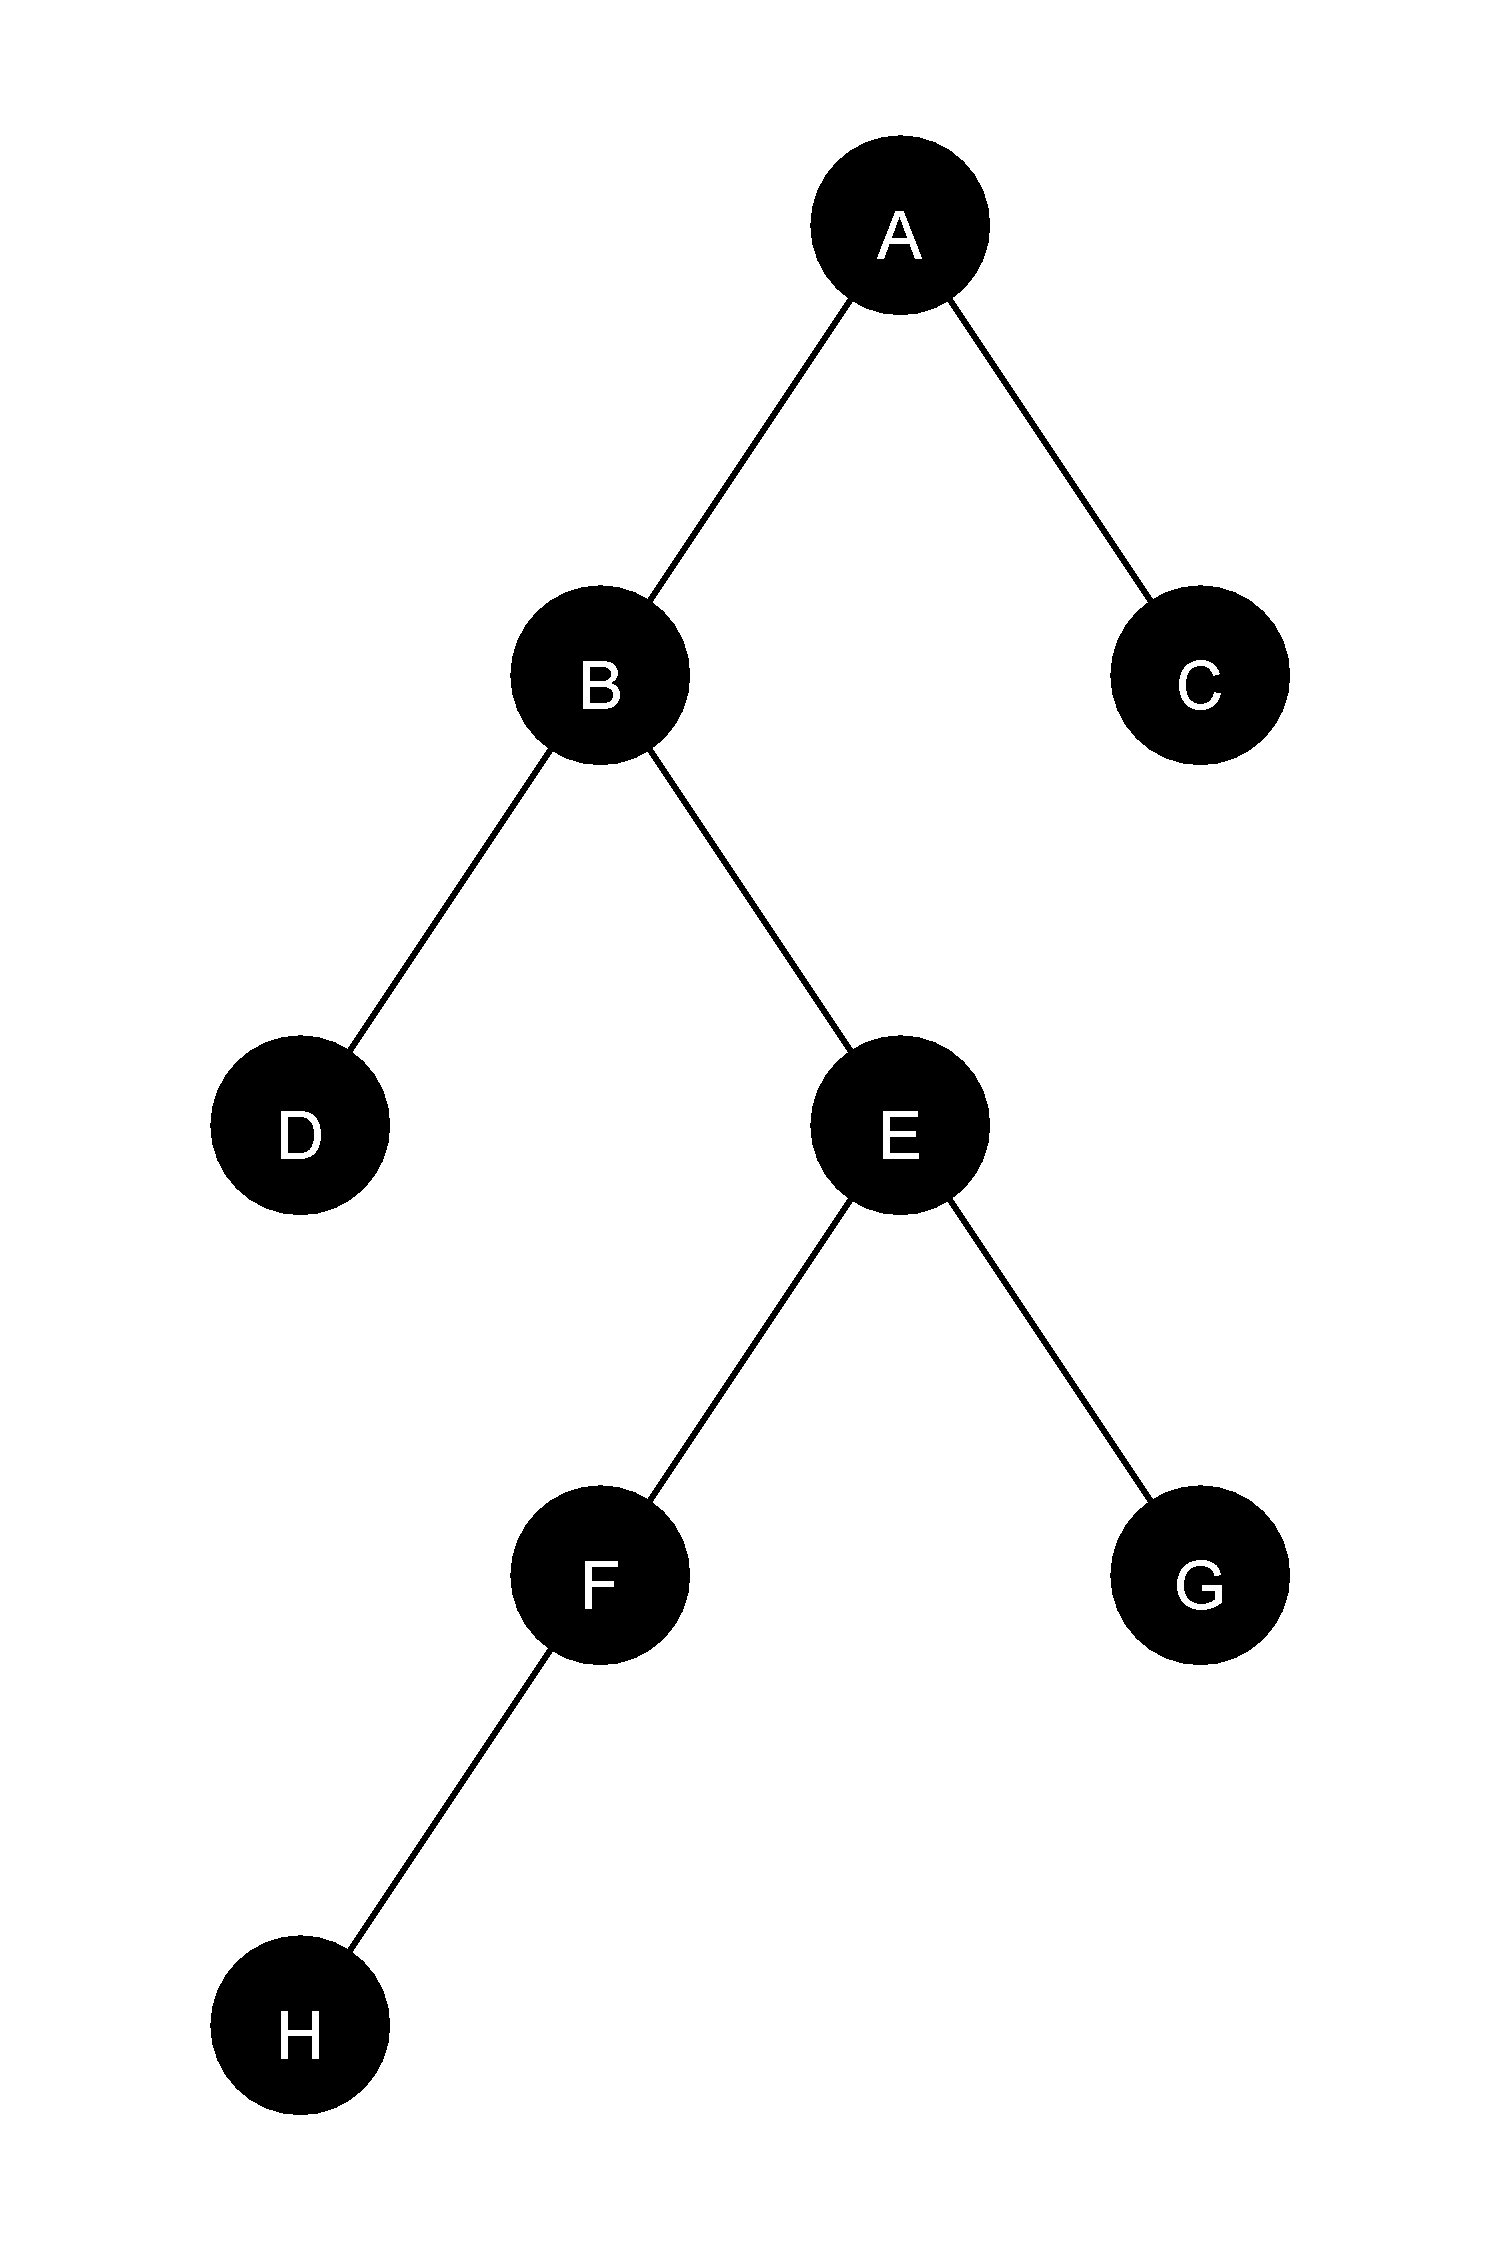
\includegraphics[scale=0.07]{abbildungen/tree_beispiel_LL_LR_RL_RR}
    \end{minipage}
    \hfill
    \begin{minipage}[]{0.65\linewidth}
        \centering
        \begin{tabular}{l | c | c | c | c | c | c | c | c}
            & A & B & C & D & E & F & G & H \\
            \hline\hline
            \textbf{LL} & H & D & C & D & H & H & G & H \\
            \textbf{LR} & G & D & C & D & F & H & G & H \\
            \textbf{RL} & C & H & C & D & G & H & G & H \\
            \textbf{RR} & C & G & C & D & G & H & G & H \\
            \end{tabular}
    \end{minipage} 
    \caption{Beispielhafte Bestimmung für LL, LR, RL, RR}
\end{figure}

Der Algorithmus zum Zeichnen von Bäumen von Reingold und Tilford lässt sich in zwei Phasen unterteilen.
Den ersten Teil stellt die Prozedur “Setup” dar. Diese Prozedur erhält vier Eingabeparameter, nämlich einen Knoten, 
die Höhe des Knotens im Gesamtbaum, sowie RMOST und LMOST. RMOST und LMOST sind jedoch nicht vom Datentyp Node, sondern 
von einem neuen Datentyp namens Extreme. Extreme sind Strukturen, die drei Attribute besitzen: 
\begin{itemize}
    \item Verweis auf einen Knoten
    \item Offset \todo{näher beschreiben} 
    \item Höhe des Knotens im Gesamtbaum
\end{itemize}

Zu Beginn der Prozedur wird geprüft, ob der übergebene Knoten NULL ist. Wenn dies nicht der Fall ist, 
dann wird die Y-Koordinate des Knotens auf seine Höhe gesetzt. Danach wird die Prozedur rekursiv aufgerufen, 
um eine Post-Order Traversierung auszuführen. Dieser Aufruf sieht wie folgt aus:

\begin{lstlisting}
    SETUP (L, LEVEL+1, LR, LL );
    SETUP (R, LEVEL+1, RR, RL );
\end{lstlisting}

Durch die Post-Order Traversierung wird die Setup Prozedur solange aufgerufen, bis der aktuelle Knoten das Blatt unten links ist. 
Da ein Blatt automatisch der am weitesten links und am weitesten rechts stehende Knoten ist, werden die Adressen von 
RMOST und LMOST auf diesen Knoten gesetzt. Außerdem wird die Höhe von RMOST und LMOST auf die Höhe des aktuellen Knotens gesetzt. 
Zudem werden die Offsets des Knotens und von RMOST sowie LMOST auf null gesetzt.

\subsection{Implementierung in Java}
\erstelltvon{Treulieb}

\begin{figure}[H]
    \centering
    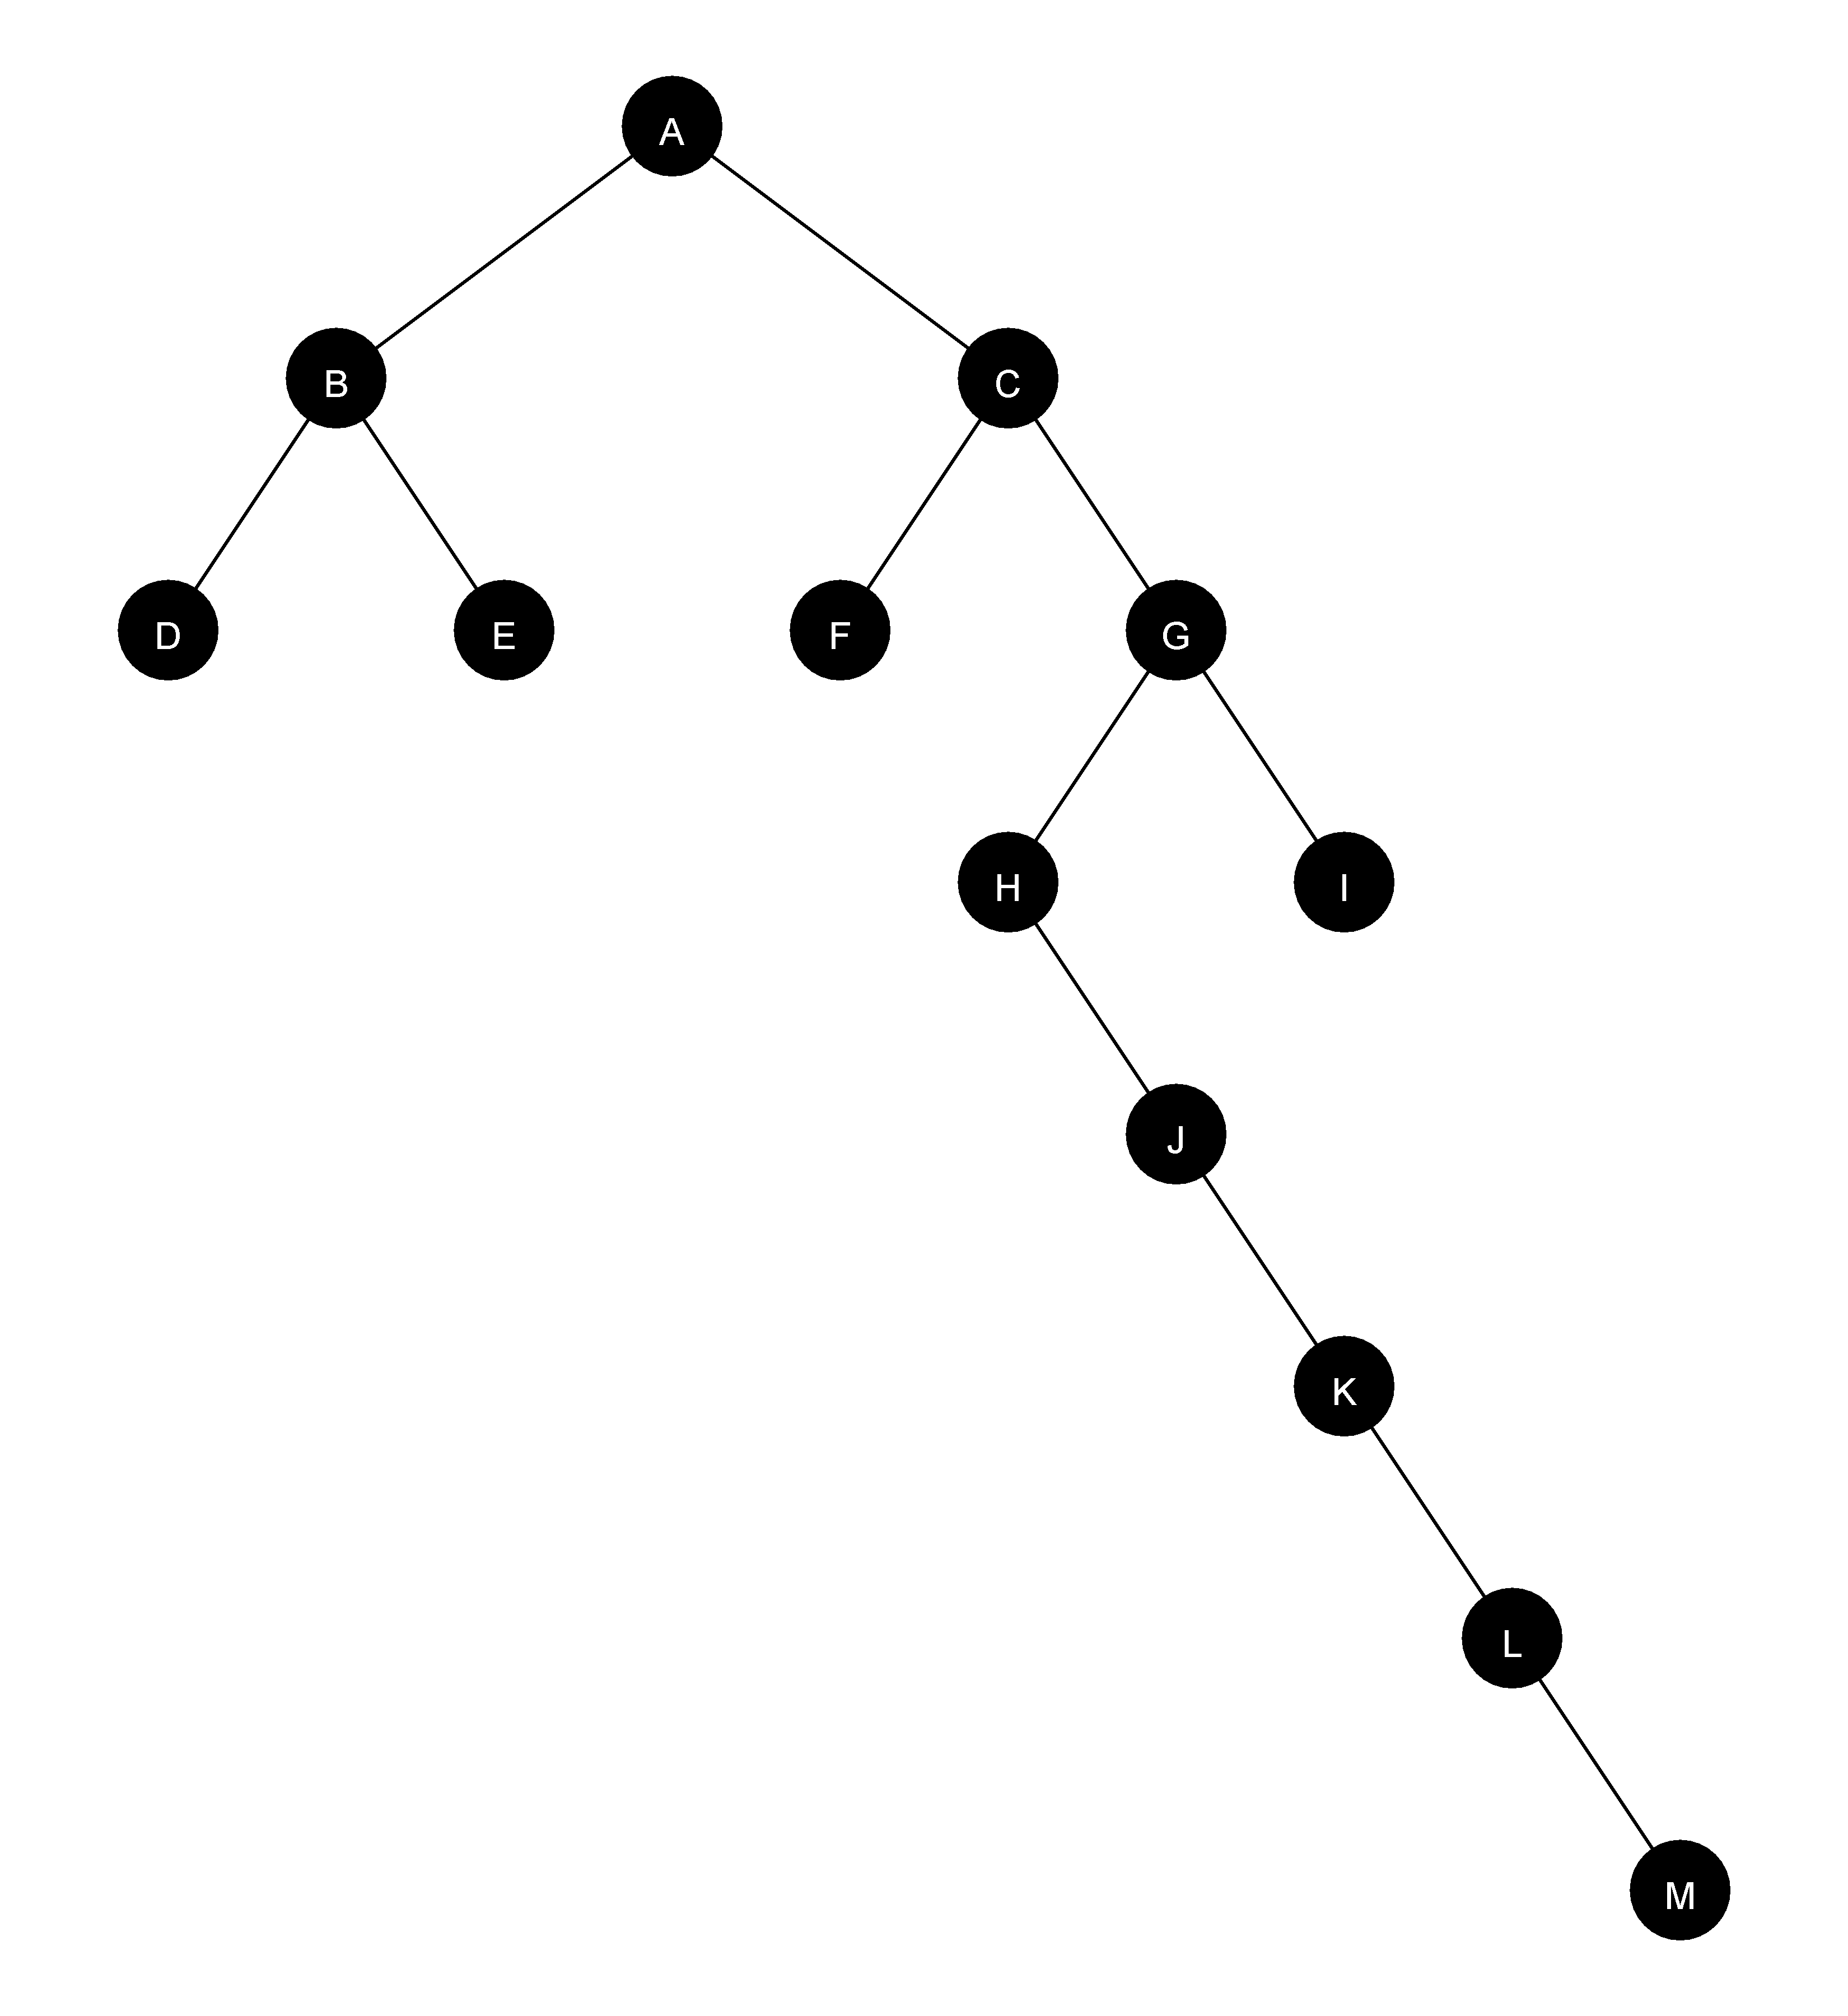
\includegraphics[scale = 0.05]{abbildungen/baum_algo_3_n1}
    \caption{Gezeichneter komplexer Baum durch den Tilford Algorithmus}
    \label{pic:baum_algo_3_n1} 
\end{figure}

\begin{figure}[H]
    \centering
    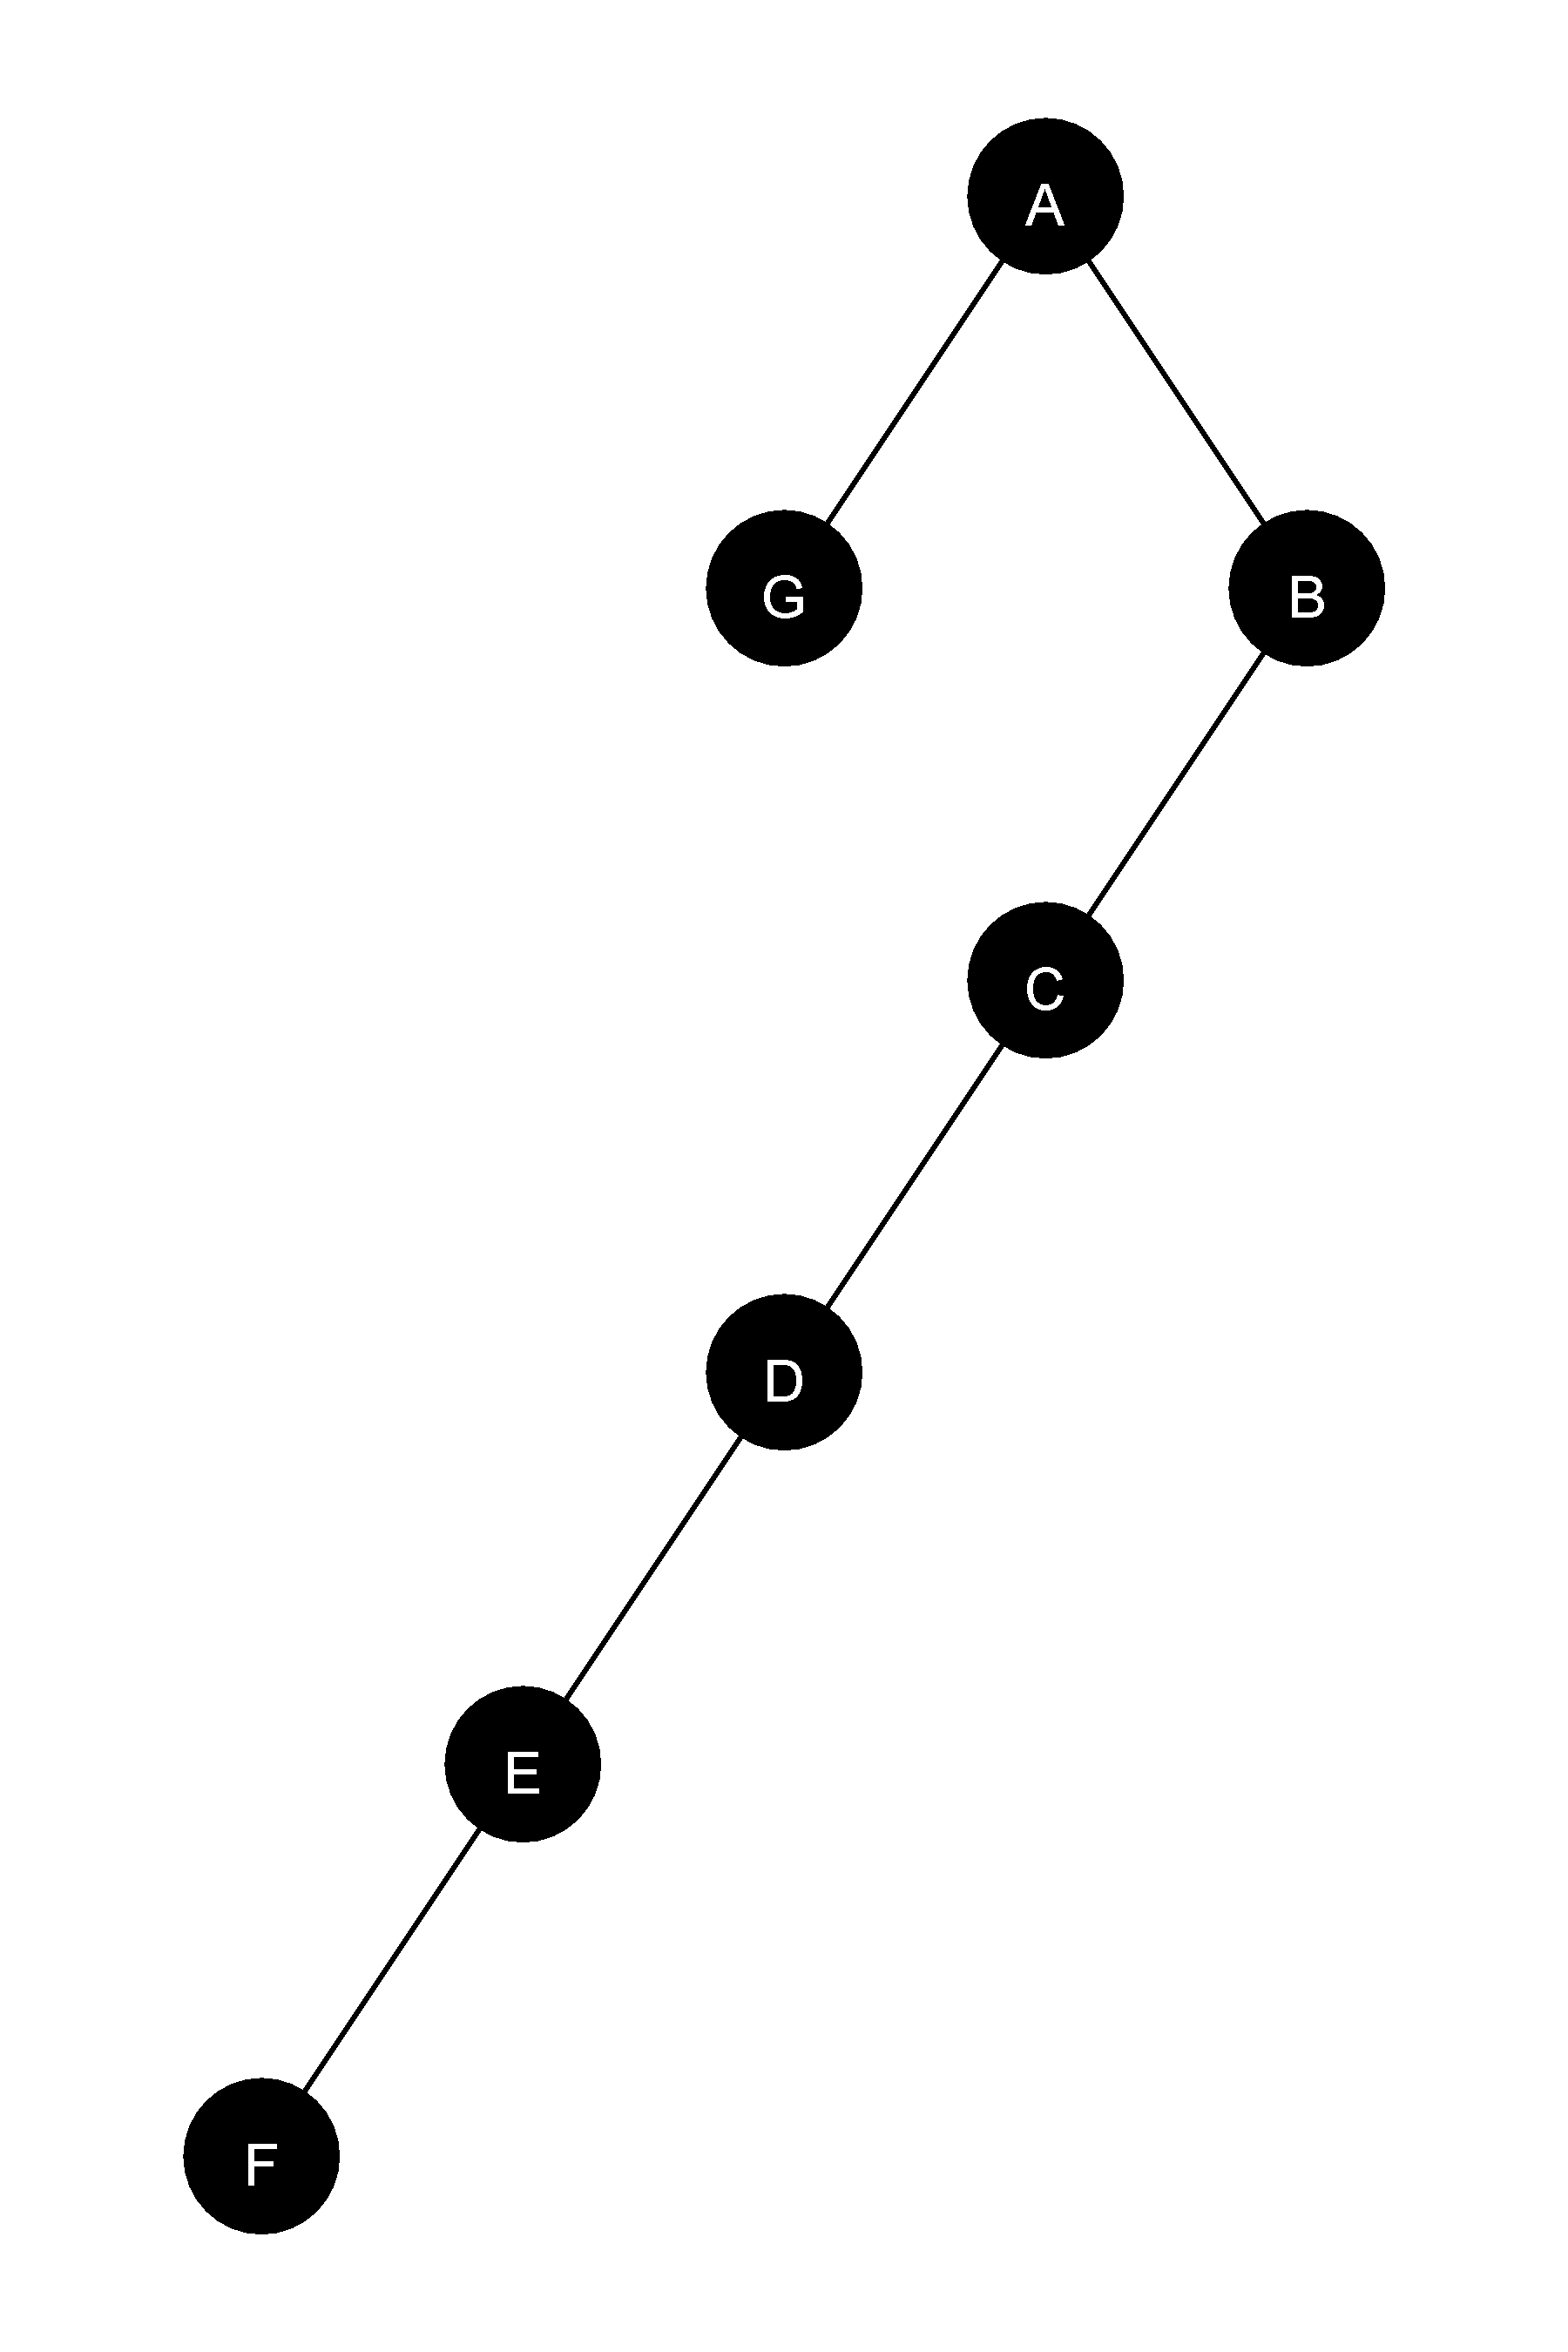
\includegraphics[scale = 0.07]{abbildungen/baum_algo_3_n2}
    \caption{Gezeichneter einfacher Baum durch den Tilford Algorithmus}
    \label{pic:baum_algo_3_n2} 
\end{figure}

Um diesen Algorithmus implementieren zu können, muss die zuvor erstellte BinaryKnoten-Klasse um ein 
Attribut erweitert werden: vom Typ Boolean mit dem Namen 'thread'. Zudem wurde eine weitere Klasse 
namens 'Extreme' definiert, die wie zuvor beschrieben, implementiert wurde. Die Extreme-Klasse sieht wie folgt aus:

\begin{lstlisting}[caption=Implementierung der Extreme-Klasse, label=code:algo3_extreme]
private static class Extreme {
    BinaryKnoten knoten;
    int offset;
    int level;
    
    void set(BinaryKnoten k, int offset) {
        this.knoten = k;
        this.level = k.getHoehe();
        this.offset = offset;
    }
}
\end{lstlisting}

Ferner wurden die zuvor beschriebenen Prozeduren 'setup' und 'petrify' implementiert. Die implementierte Prozedur
'setup' unterscheidet sich zum zuvor beschriebenen Ablauf. Sie wird nun nicht mehr rekursiv aufgerufen und besitzt 
nur einen Eingabeparameter, den Wurzelknoten. Hiernach wird mithilfe der 'traversPostOrder'-Methode aus der 
BinaryKnoten-Klasse über den Baum traversiert.

\begin{lstlisting}[caption=Ausschnitt aus der setup-Prozedur, label=code:algo3_setup]
public static void setup(BinaryKnoten wurzel) {
    // Initialisierungen von Variablen
    // <...>
    // Ueber den Baum in der Post-Order traversieren
    wurzel.traversPostOrder(k -> {
        BinaryKnoten knoten = (BinaryKnoten) k;

        // Bestimmen der Y-Koordinate
        knoten.setY(2 * knoten.getHoehe() + 1);

        // Vorlaeufige relative X-Koordinate bestimmem
        // <...>
    }
}
\end{lstlisting}

Abweichend zum Ablauf entspricht die Y-Koordinate nicht der Höhe des Knotens. Stattdessen wird diese wie im 
Ablauf aus dem Kapitel \ref{chap:kapitel3_1_Ablauf} berechnet. Dies bietet den Vorteil, 
dass die Methodik zum Zeichnen der Bäume nicht verändert werden muss. Die weitere Implementierung folgt 
der Beschreibung aus dem Ablauf.

Die Implementierung der Prozedur 'petrify' entspricht der Beschreibung aus dem Ablauf.

Hiernach wurde die Prozedur 'algorithmus3' definiert. Diese ruft zu Beginn die beiden Prozeduren, 
'setup' und 'petrify' auf. Danach müssen die X-Koordinaten noch angepasst werden, da diese 
negativ sein können. Hierfür wird der kleinste X-Wert ermittelt, dessen absoluter Wert 
addiert mit eins in der Variable 'offset' gespeichert wird. Nun werden alle X-Koordinaten des 
Baums mit dem Wert aus 'offset' addiert. 

Zwei beispielhafte Ergebnisse können in den Abbildungen \ref{pic:baum_algo_3_n1} 
und \ref{pic:baum_algo_3_n2} betrachtet werden. 


\subsection{Vor- und Nachteile}
\erstelltvon{Garan}
Ein Algorithmus, welcher Aesthetic 4 erfüllt, kann Bäume produzieren, welche nicht maximal schmal sind. 
Für Reingold und Tilford ist das Erfüllen dieser Anforderung jedoch wichtiger als das Einhalten des physikalischen Limits, 
da Aesthetic 4 dafür sorgt, dass diese Bäume für Menschen übersichtlicher und leichter zu verstehen sind.\cite[]{q2} Dafür ist der Algorithmus 
jedoch auch der am komplexesten zu verstehen und implementieren ist. Als Ausgleich produziert dieser Algorithmus aber auch das beste Ergebnis
im Vergleich zu den beiden Algorithmen von Wetherell und Shannon. Selbst bei komplexeren Bäumen, wie in Abbildung \ref{pic:baum_algo_3_n2},
wird ein übersichtlicher und ästhetisch ansprechender Baum gezeichnet. 

Ähnlich wie der verbesserte Algorithmus von Wetherell und Shannon ist der Algorithmus von Reingold und Tilford so wie er ist nur in Lage
Binärbäume zu zeichnen. Jedoch beschreiben die beiden Autoren wie der Algorithmus modifiziert werden kann um beliebige Bäume zu zeichnen.

